\subsection{Обработка контроля минимальных остатков ключевых позиций}
\subsubsection{Описание и настройка}
\begin{itemize}	
	\item Для контроля минимальных остатков по ключевым позициям в разрезе магазинов, создана соответствующая обработка.\par
	Обработка предназначена для запуска в двух режимах - "<автоматическом"> и "<административном">.	\par
			\sidenote[-2ex][]{Принимаются замечания и пожелания}.
	В "<автоматическом"> режиме обработка настроена следующим образом: Запуск обработки происходит при старте системы. При запуске проверяется пользователь, есть ли он в списке тех для кого предназначен данный отчет и если есть происходит проверка, показывалось ли сегодня ему сообщение о критических остатках ключевых позиций и если нет и остатки ниже установленных значений, то появляется таблица со списком номенклатуры и остатками, при этом показываются только остатки по текущему магазину.	\par
	\begin{figure}[H]
		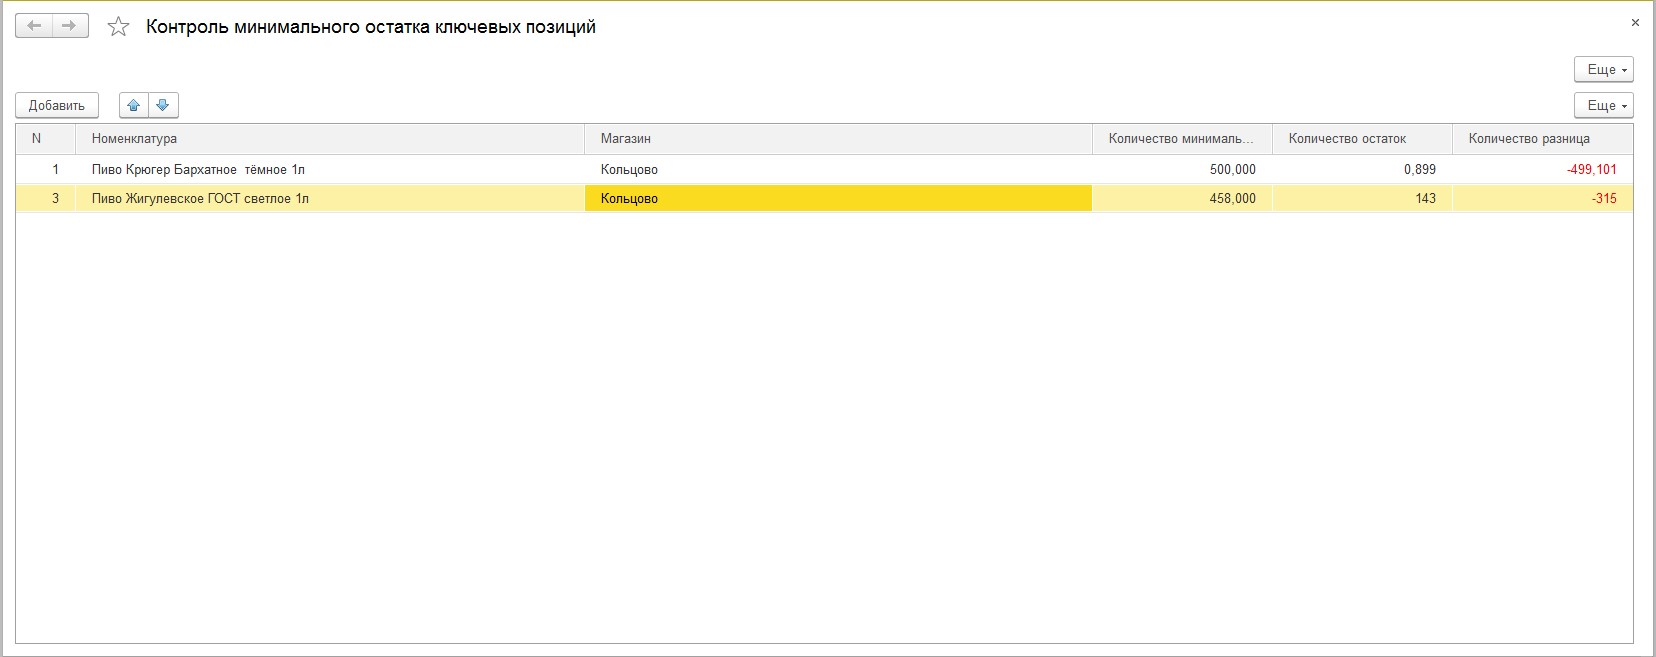
\includegraphics[width=0.90\textwidth]{10_1.jpg}
		\caption{Старт при запуске системы.}
		\label{ris:10_1.jpg}
	\end{figure}
	В "<Административном">  режиме обработка  запускается в центральном узле, из интерфейса пользователя.
	\begin{figure}[H]
		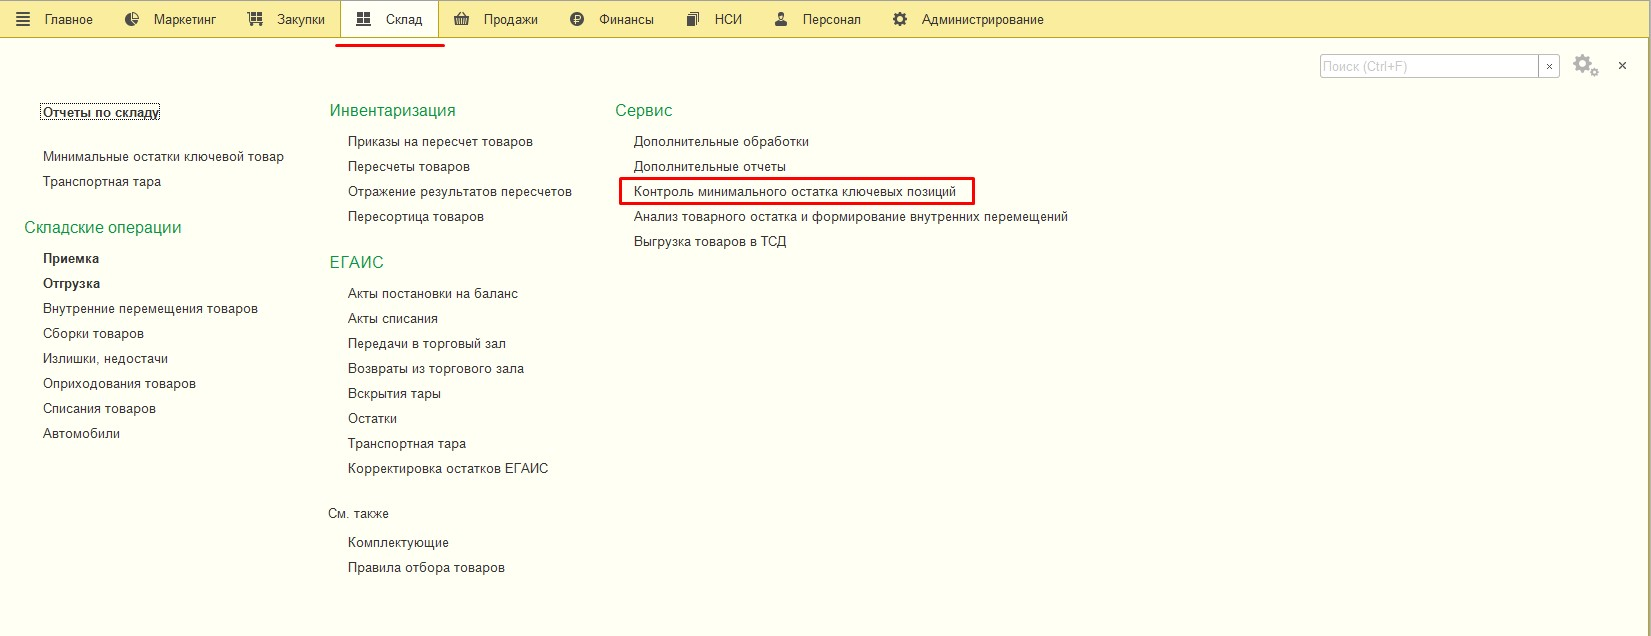
\includegraphics[width=0.90\textwidth]{10_2.jpg}
		\caption{Обработка "<Контроль минимальных остатков ключевых позиций">}
		\label{ris:10_2.jpg}
	\end{figure}
	 При таком способе запуска отбора по магазинам не происходит и есть возможность увидеть критические остатки ключевой номенклатуры по всем магазинам. Обработка находится в подсистеме "<Склад"> в разделе "<Сервис">
	\begin{figure}[H]
		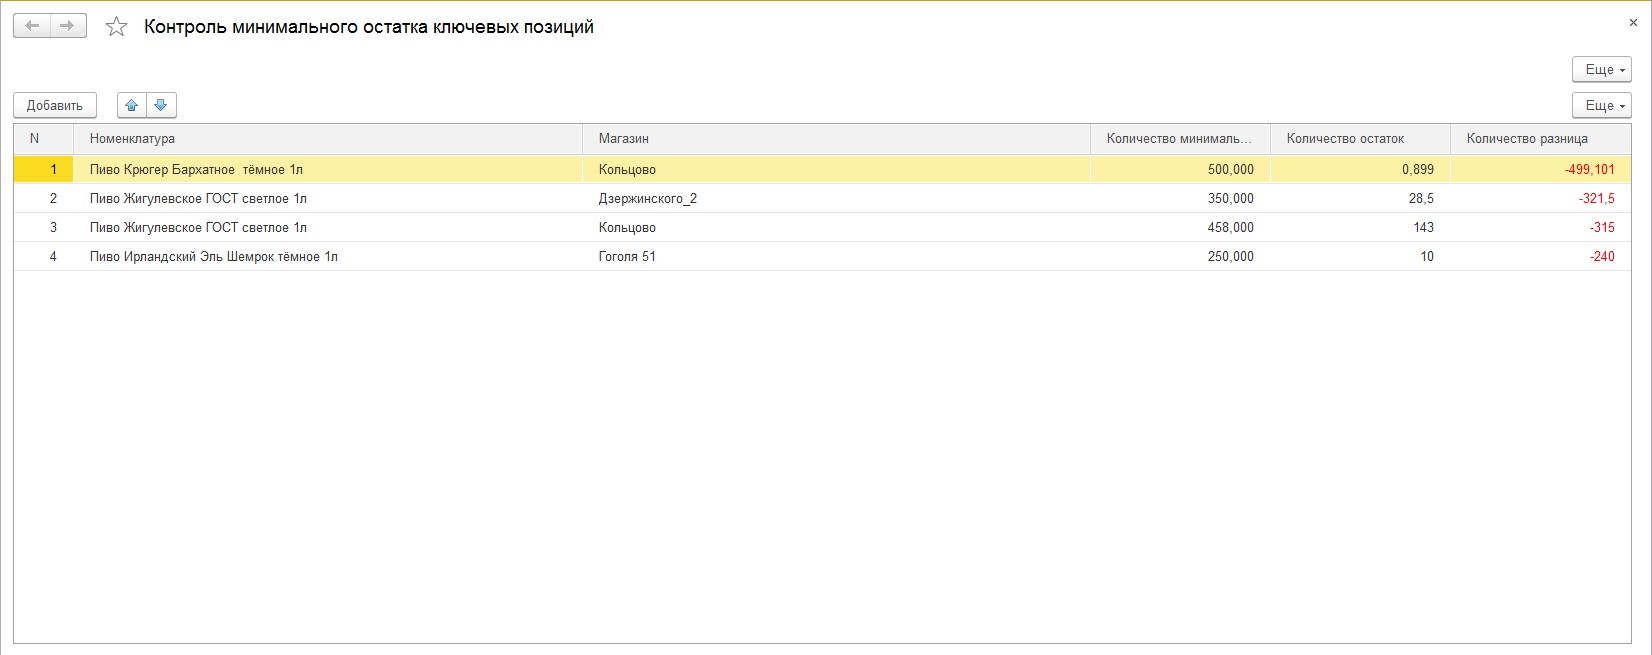
\includegraphics[width=0.90\textwidth]{10_3.jpg}
		\caption{Обработка в "<Административном"> режиме}
		\label{ris:10_3.jpg}
	\end{figure}

	\item Перед началом работы необходимо внести минимальные остатки по ключевым позициям. Для этого в подсистеме "<Склад">
		  выбрать "<Минимальные остатки ключевой товар">.
  	\begin{figure}[H]
		  	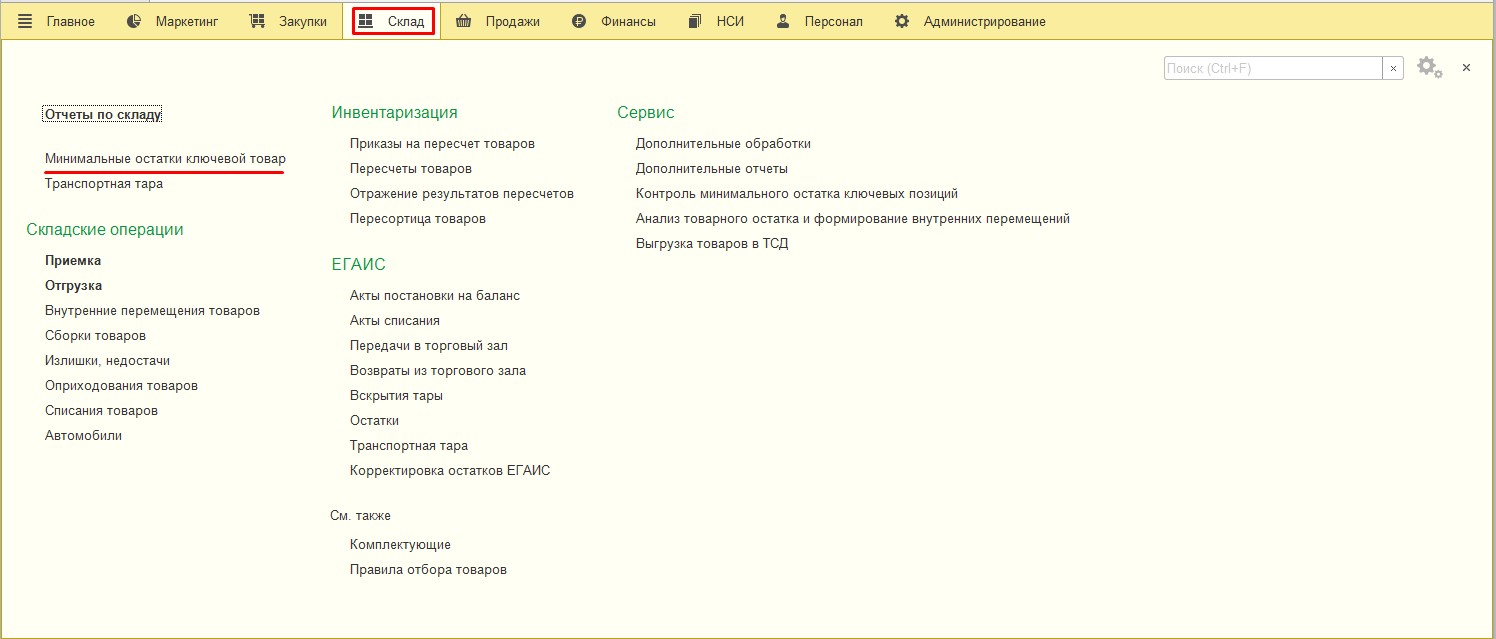
\includegraphics[width=0.99\textwidth]{10_7.jpg}
		  	\caption{Минимальные остатки ключевой товар.}
		  	\label{ris:10_7.jpg}
  \end{figure}
	\item С помощью \keys{Создать}  добавить запись. 
  	\begin{figure}[H]
		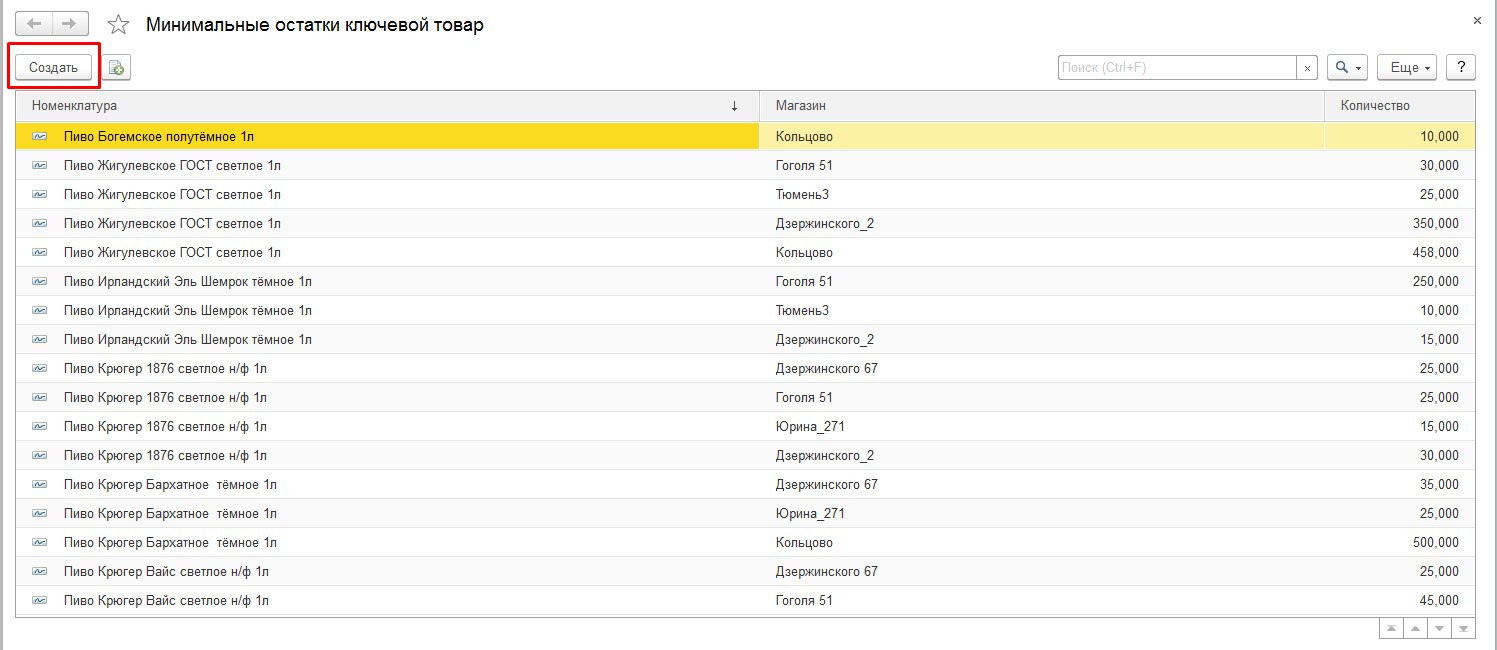
\includegraphics[width=0.99\textwidth]{10_8.jpg}
		\caption{Добавление записи.}
		\label{ris:10_8.jpg}
	\end{figure}
	\item Указать номенклатуру, магазин и количество.	
  	\begin{figure}[H]
		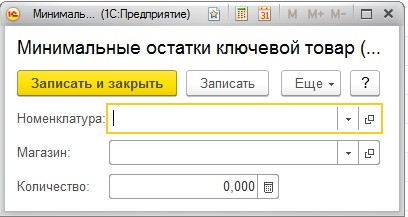
\includegraphics[width=0.5\textwidth]{10_9.jpg}
		\caption{Заполнение реквизитов.}
		\label{ris:10_9.jpg}
	\end{figure}
	\item Для автоматической работы этого отчета необходимо в каждом узле произвести настройку. Для этого в подсистеме "<Администрирование">  нужно открыть "<Учет сообщений пользователю">
	\begin{figure}[H]
		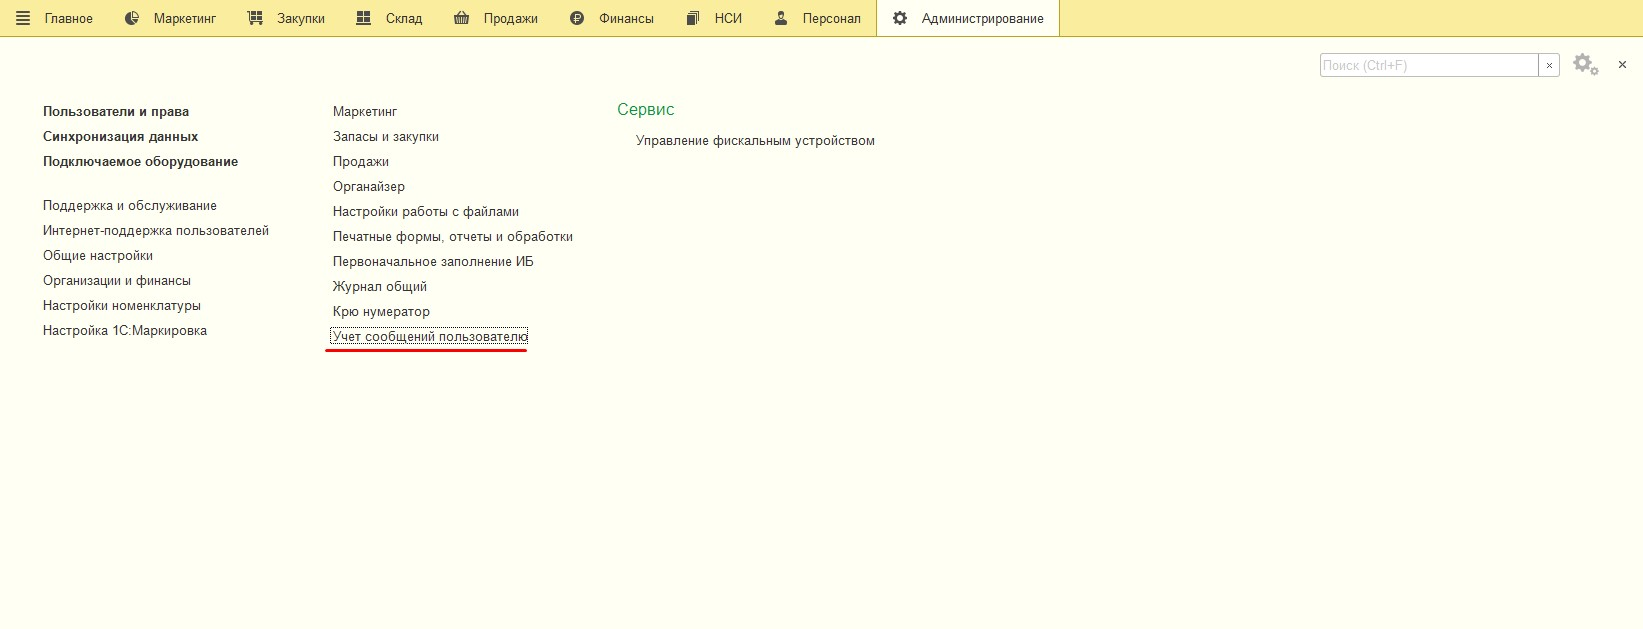
\includegraphics[width=0.99\textwidth]{10_4.jpg}
		\caption{Учет сообщений пользователю.}
		\label{ris:10_4.jpg}
	\end{figure}
	\item И с помощью кнопки \keys{Создать}  добавить пользователей для которых в данном узле необходимо организовать сообщение о снижении минимального остатка.
	\begin{figure}[H]
		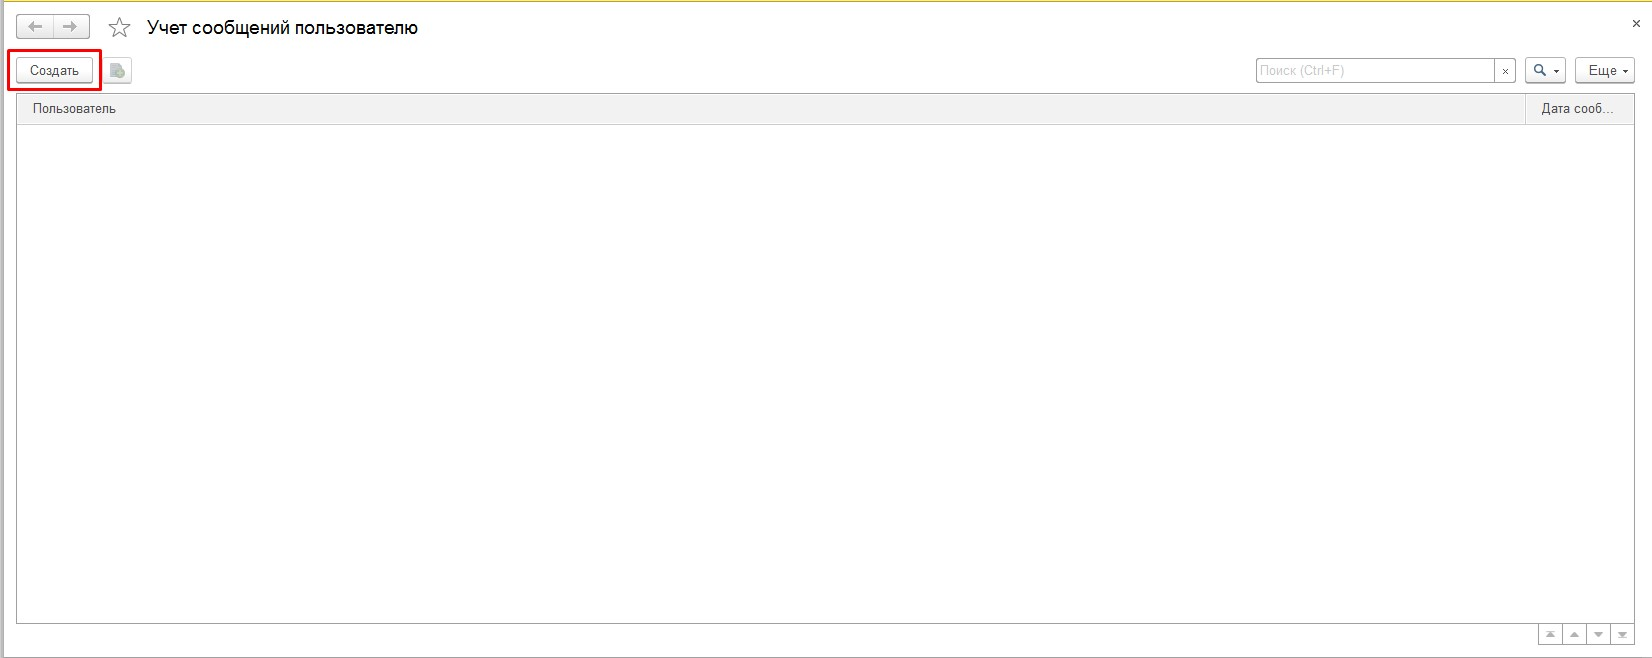
\includegraphics[width=0.99\textwidth]{10_5.jpg}
		\caption{Создать записи.}
		\label{ris:10_5.jpg}
	\end{figure}
	\item Дату необходимо указать любую старше дня когда вы заводите запись.
	\begin{figure}[H]
		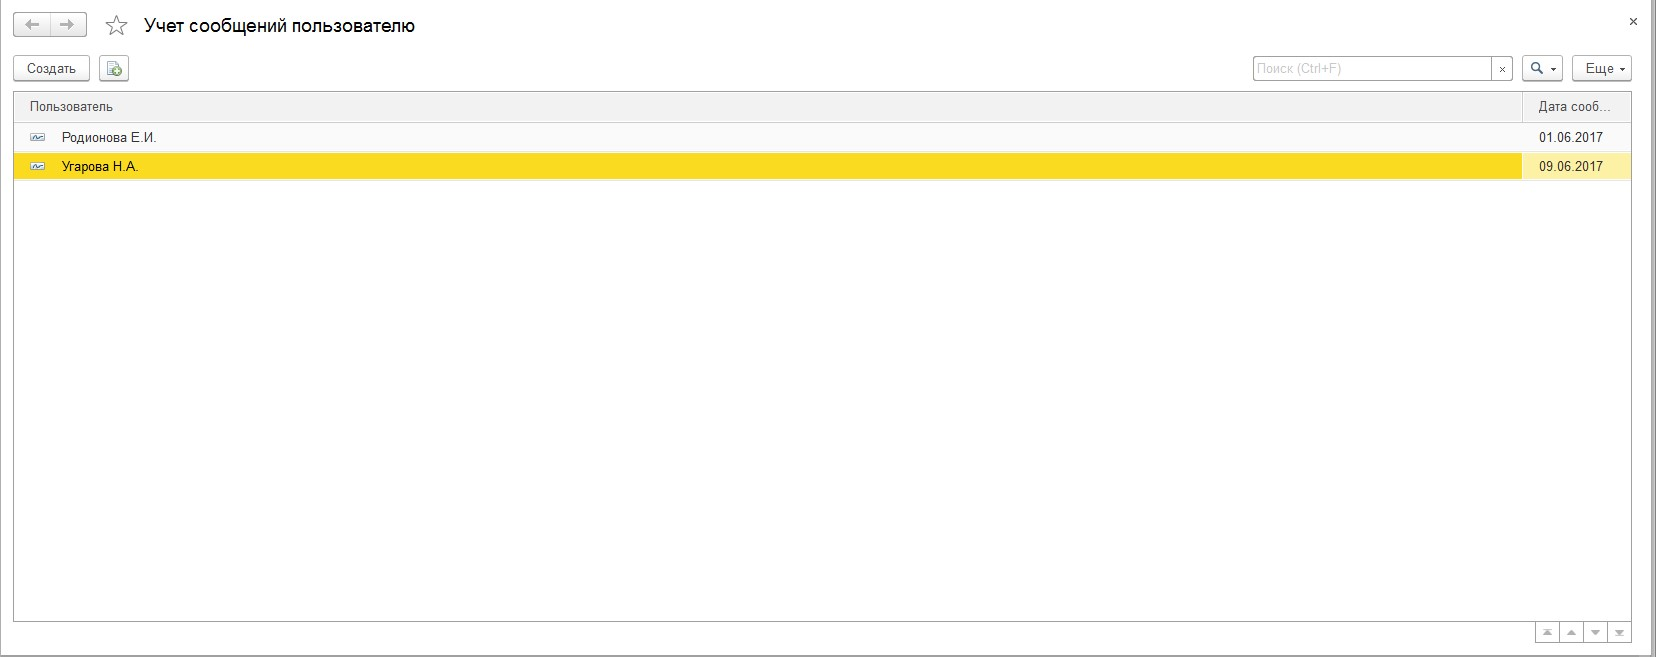
\includegraphics[width=0.99\textwidth]{10_6.jpg}
		\caption{Соданные записи.}
		\label{ris:10_6.jpg}
	\end{figure}	
	\item После этого, при запуске под указанным пользователем обработка запустится и если будет номенклатура с критическим остатком выведет список с остатками. Если все остатки будут нормальными, то пользователь не увидит ни каких сообщений.

\end{itemize}